% MX17 Paper II -- reconstruction. Outline stage.
% Journal and author list undecided (PAPER_PLAN C4): plain article for now; switch
% the class (elsarticle for NIM A, jinst for JINST) once chosen.
\documentclass[11pt,a4paper]{article}
\usepackage[margin=2.2cm,marginparwidth=2.6cm]{geometry}
\usepackage[T1]{fontenc}
\usepackage{lmodern}
\usepackage{amsmath,amssymb}
\usepackage{graphicx}
\usepackage{booktabs}
\usepackage{siunitx}
\usepackage{authblk}
\usepackage[hidelinks]{hyperref}
\usepackage{cleveref}
\usepackage{drafting}
% \draftnotesfalse   % uncomment for a clean read without notes

\graphicspath{{figures/}}

\title{Reconstructing micro-TPC tracks on resistive strips: why hit times fail, and a waveform forward model}
\author{\tbw{author list -- undecided (C4)}}
\date{Outline draft, \today}

\begin{document}
\maketitle

\begin{abstract}
\tbw{Abstract written last. Key points: on resistive strips a per-strip hit time mixes in delayed copies of the
neighbours' charge (sharing kernel measured head-on in the SPS beam), compressing the drift-time ladder by 20--30\,\%
for every estimator; a forward model fitted to the waveforms removes the bias and improves $\sigma_\theta$ on every
plane; how much a hit-based readout can recover, and what it must record.}
\end{abstract}

\ifdraftnotes
\listoftodos[Open items]
\clearpage
\fi

\section{Introduction}\label{sec:intro}
\sectionstate{open}{\texttt{RECONSTRUCTION\_BASIS.md}; \texttt{WAVEFORM\_FIRST\_THREADING.md}}
\intent{Micro-TPC angles from per-strip hit times are standard. On resistive strips they are biased in a way no
threshold or estimator fixes. This paper measures why, gives the fix (a waveform forward model), and asks how
much a hit-only readout (e.g.\ VMM) can recover. Short detector summary; the rest is in~\cite{paperI}.}

\tbw{Short chamber summary: 30\,mm drift, 0.78\,mm pitch, resistive strips, DREAM sampling. Data: June cosmic bench
(five chambers, M3 reference) and det4 in the SPS H4 beam.}

\section{Signal formation on resistive strips: the sharing kernel}\label{sec:kernel}
\sectionstate{ready}{\texttt{sps\_beam\_test\_26/analysis/sharing\_kernel}, \texttt{angled\_kernel}, \texttt{plane\_ratio/FINDINGS.md}; \texttt{cloud\_basics} \S27--34}
\intent{Measure, model-free and head-on in the beam, how a strip's charge reaches its neighbours: amplitude and delay
to $\pm1$ and $\pm2$, gain-invariant, rotation-invariant, attachment-proof. The physical requirement $c_2<c_1$.}

\tbw{Y: $c_2/c_1$ = 0.42--0.47 at three fields; $\pm1$ delay $\sim$49\,ns; gain-invariant to 1--3\,\% (run\_66);
survives a 25.6\textdegree{} rotation. X: $\pm2/\pm1\approx$ 0.15--0.20 on all five chambers, against 0.36--0.54 in Y.
det4 $D_{RC}$ = $2.2\times10^{-4}$ ($\pm$10\,\%) in the beam. $\tau$ and $c_2$ are bounds: the tail outlasts the 3.84\,\textmu s window.}
\analysis{X-width}{the X-width excess (cloud\_basics \S28--34) is unsolved: state it as a limitation or explain it}
\askStephan{Expected RC constant of the resistive strips through the insulator (sheet resistance, kapton thickness): does $D_{RC}$ match the design?}
\begin{figure}[t]
  \centering
  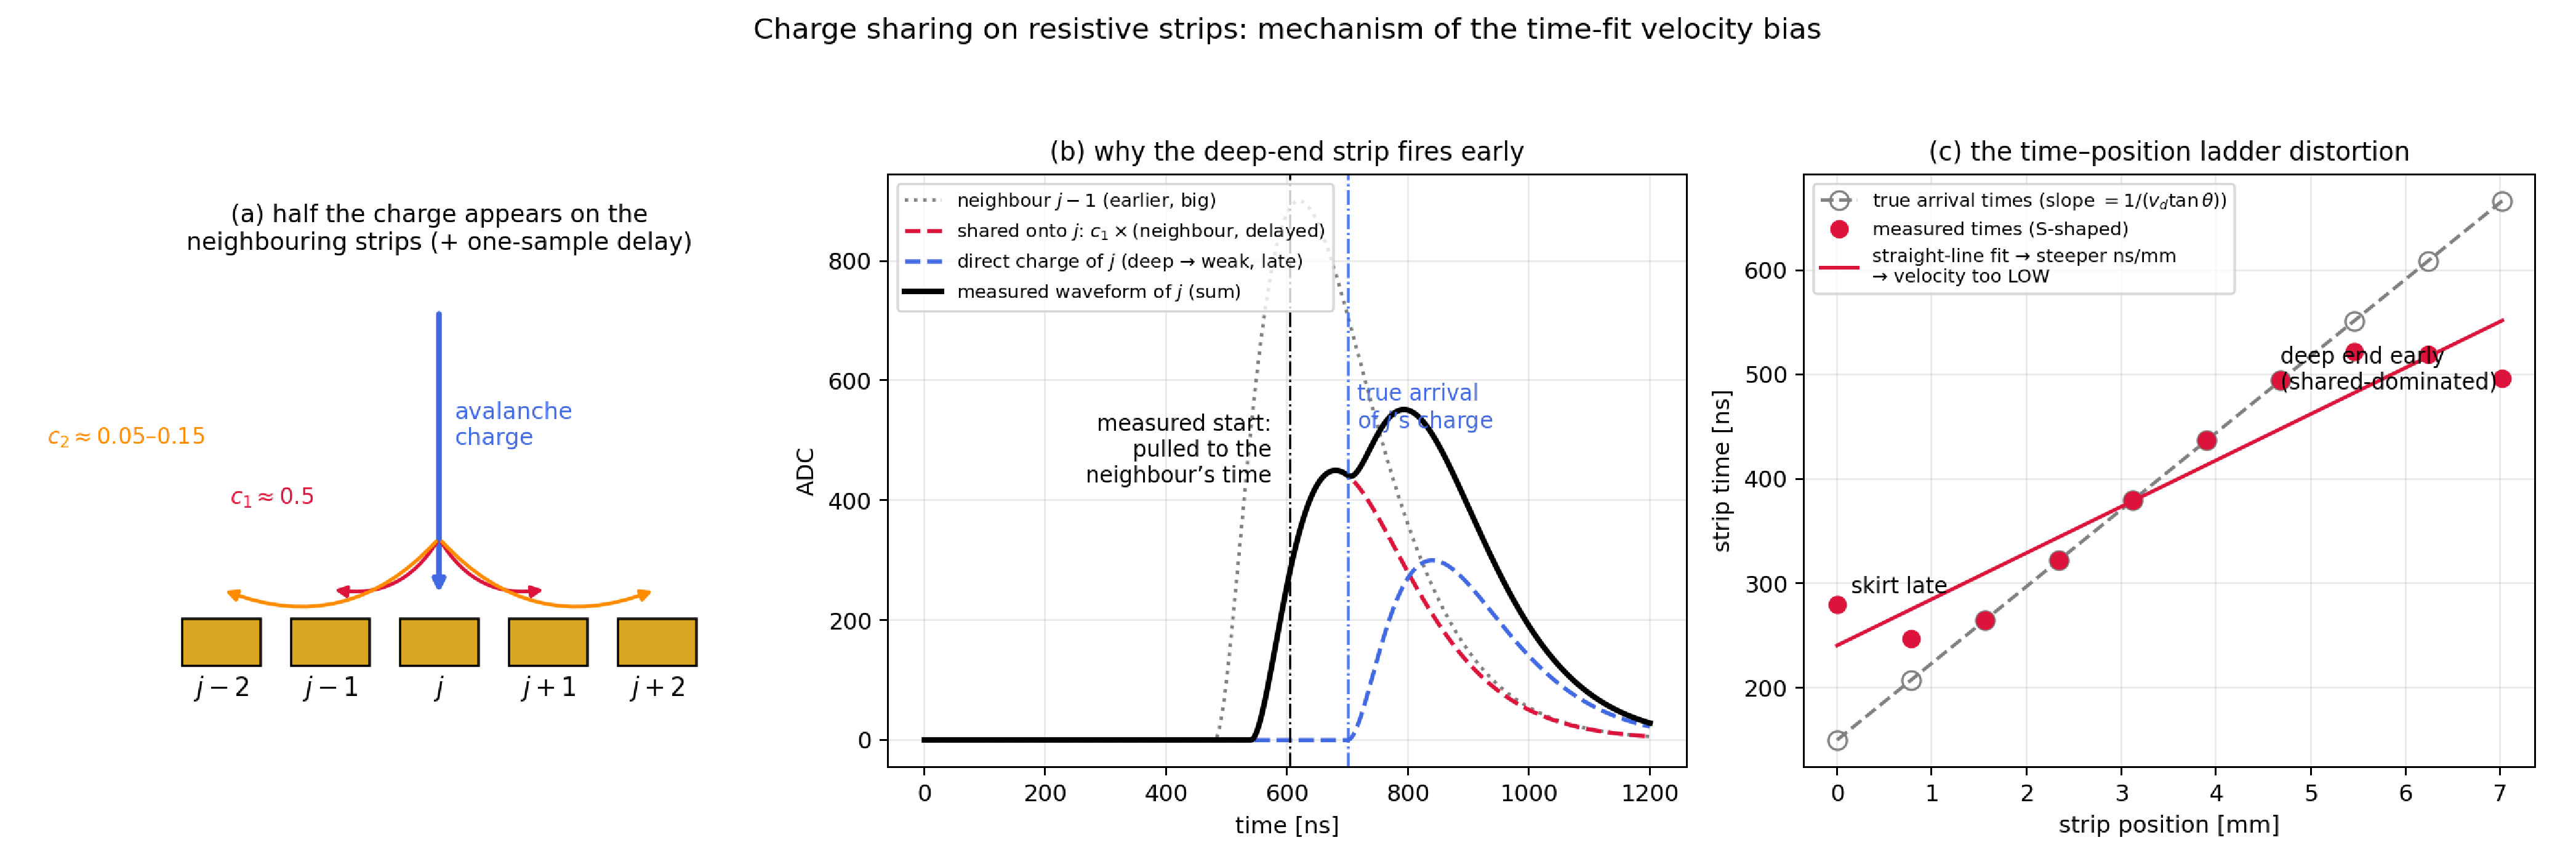
\includegraphics[width=0.7\linewidth]{sharing_cartoon}
  \caption{\tbw{How charge reaches the neighbouring strips.}}
  \label{fig:sharing_cartoon}
\end{figure}
\begin{figure}[t]
  \centering
  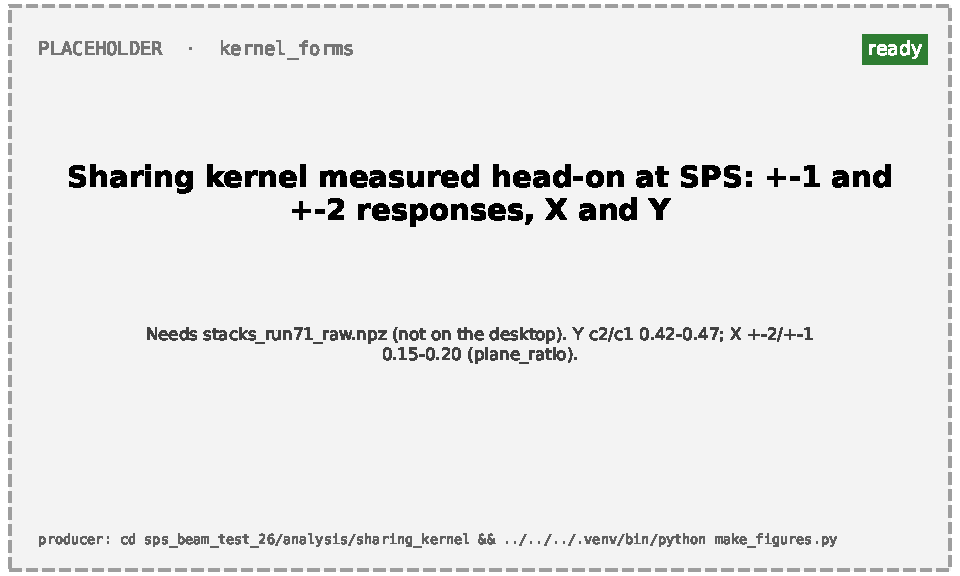
\includegraphics[width=0.9\linewidth]{kernel_forms}
  \caption{\tbw{Kernel forms measured head-on, X and Y.}}
  \label{fig:kernel_forms}
\end{figure}
\begin{figure}[t]
  \centering
  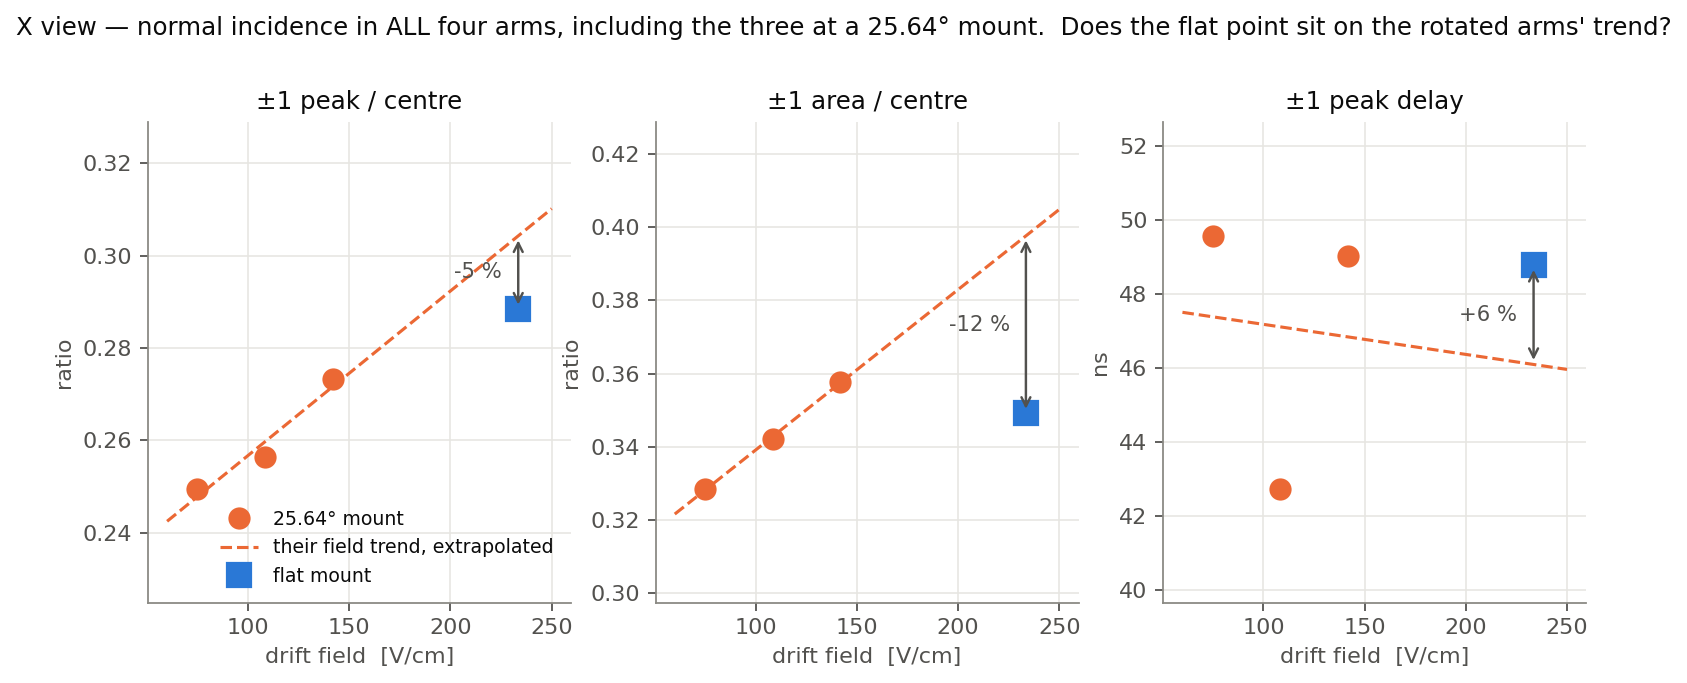
\includegraphics[width=0.7\linewidth]{angled_kernel}
  \caption{\tbw{The kernel at a 25.6 degree rotation.}}
  \label{fig:angled_kernel}
\end{figure}

\section{Why hit times fail}\label{sec:hitsfail}
\sectionstate{partial}{\texttt{WAVEFORM\_FIRST\_THREADING.md} \S3 (det3); \texttt{THREADING\_DISPLAYS\_2026-07-28.md}; fleet extension R1}
\intent{Each per-strip hit time is an aggregate of the strip's own charge and delayed copies of its neighbours'
($\sim$29\,\% at $\tau\approx47$\,ns to $\pm1$). The drift-time ladder is compressed by 20--30\,\%, reads $\sim$4\textdegree{}
too steep, and the cluster fans away from the track with depth, for rising-edge, CFD and matched-filter times alike.}
\analysis{R1}{hit tiers on r06 for all five chambers}
\begin{figure}[t]
  \centering
  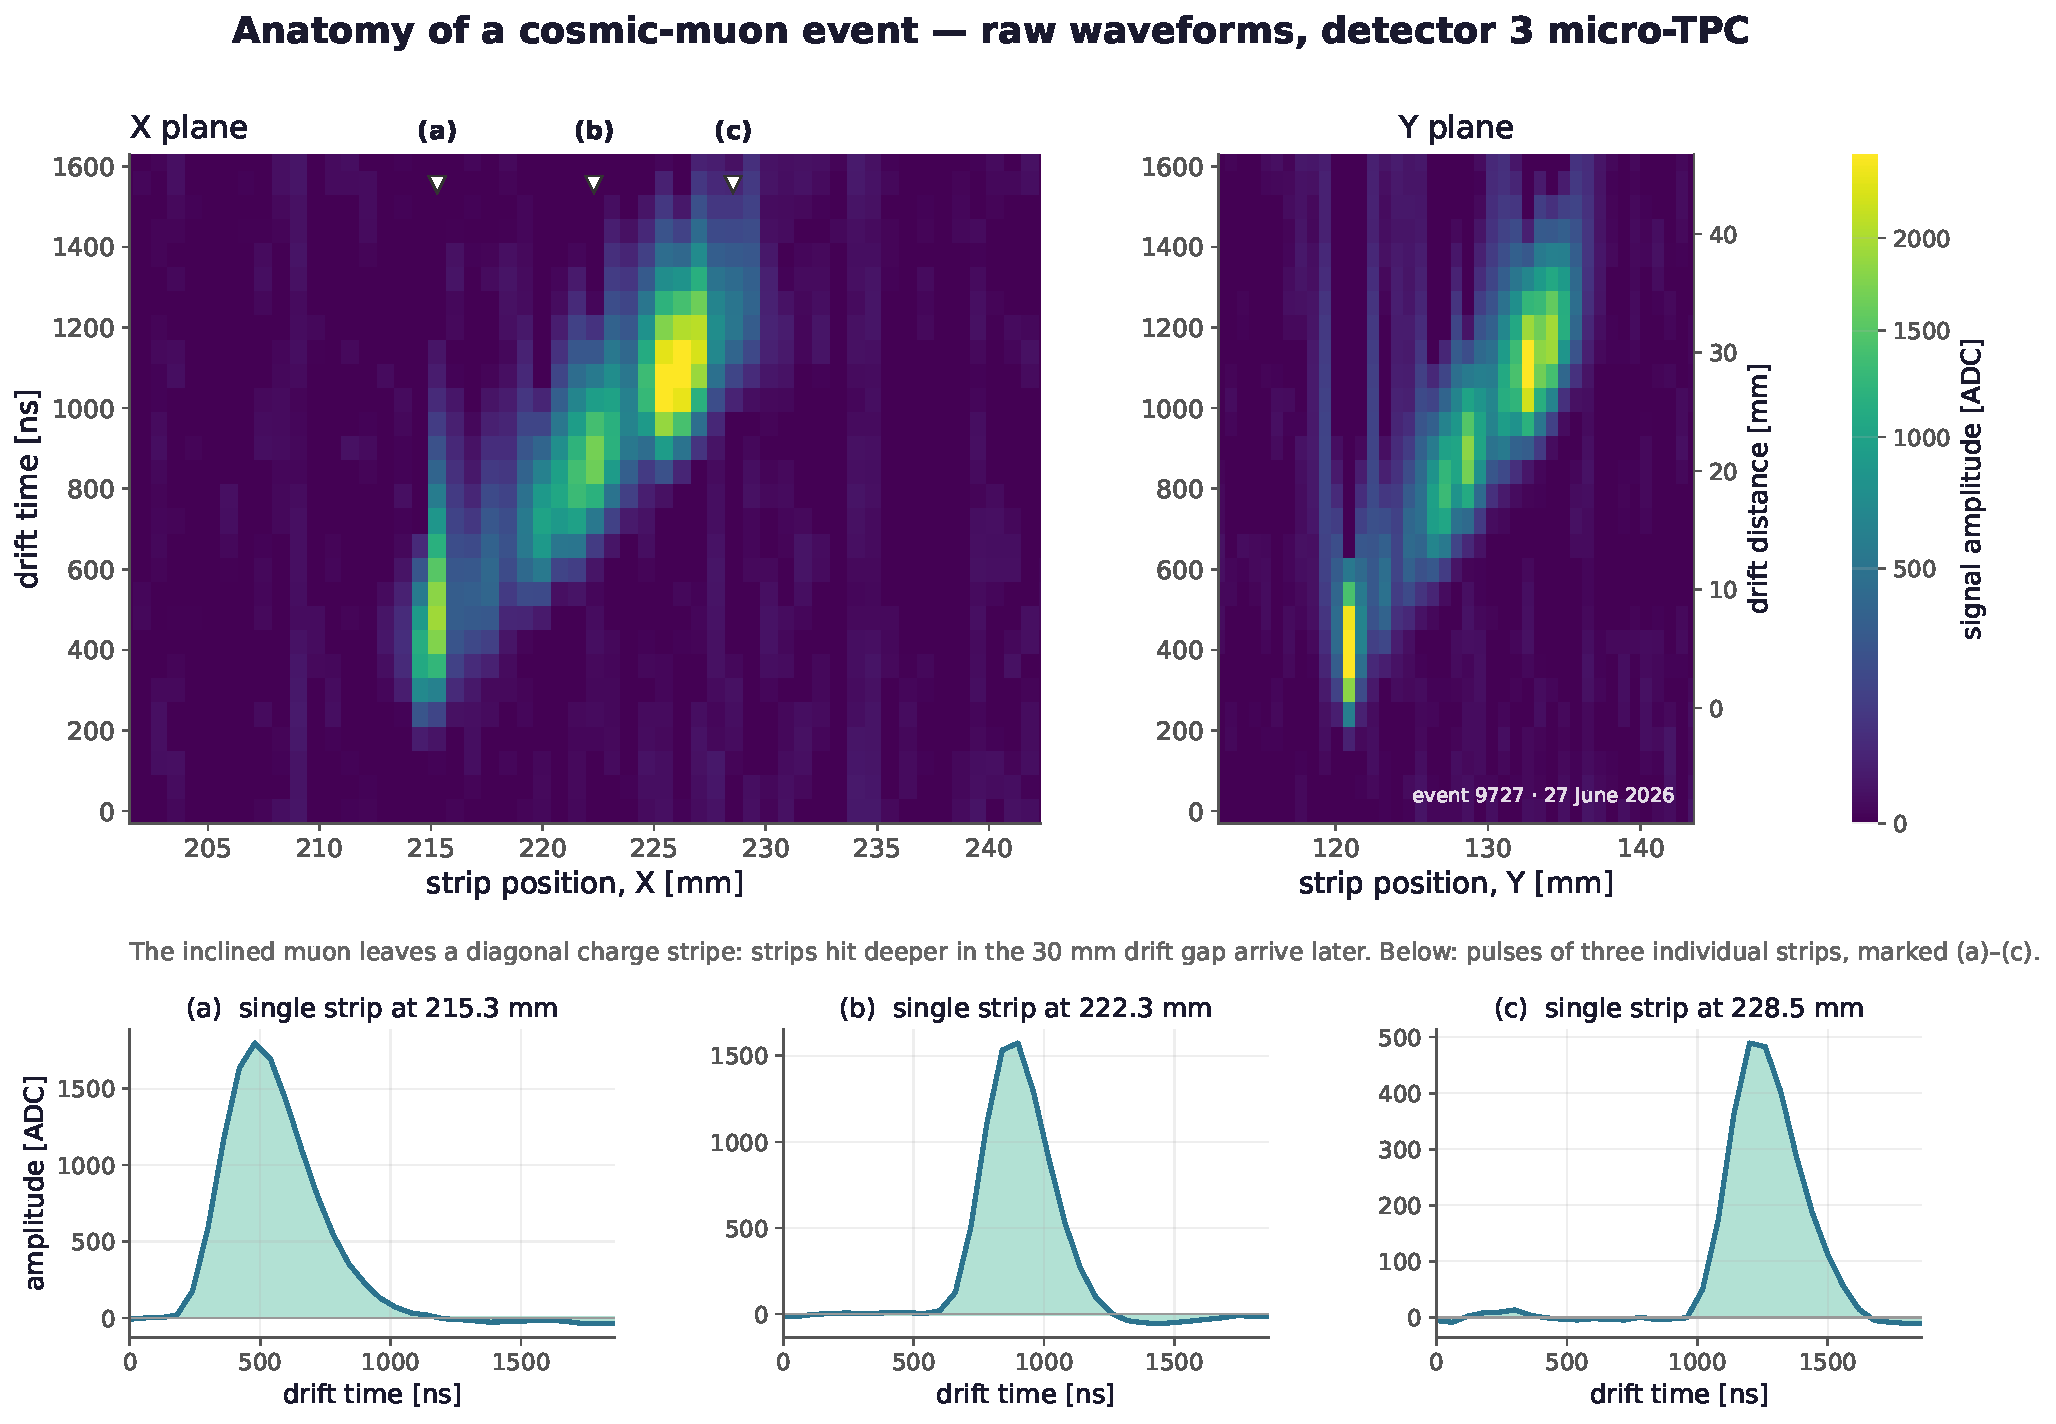
\includegraphics[width=0.85\linewidth]{event_waveforms}
  \caption{\tbw{The strip waveforms of one cosmic track.}}
  \label{fig:event_waveforms}
\end{figure}
\begin{figure}[t]
  \centering
  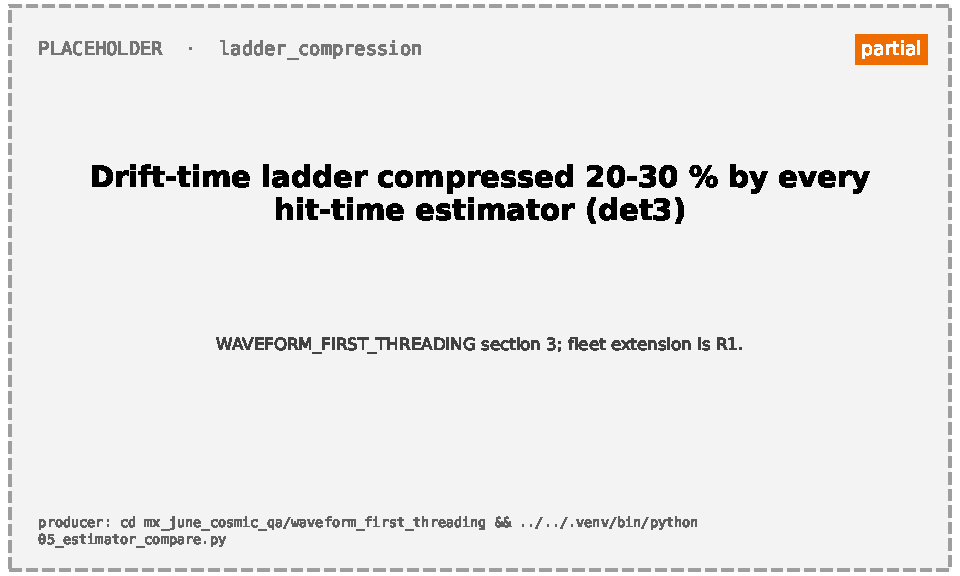
\includegraphics[width=0.8\linewidth]{ladder_compression}
  \caption{\tbw{The drift-time ladder from hit times, per estimator, against the reference.}}
  \label{fig:ladder_compression}
\end{figure}

\section{The waveform forward model and its calibration}\label{sec:model}
\sectionstate{ready}{\texttt{WAVEFORM\_FIRST\_THREADING.md} \S4, \S9, \S15; \texttt{wft/}; R9 (calibration protocol)}
\intent{The model (per-plane pulse template, sharing kernel, drift and diffusion), the fit, and the calibration
protocol with its traps: per detector and per run condition; kernel ordering enforced
(\texttt{check\_kernel\_ordering}); $v$ from the kernel hyperfit, never from a Magboltz prior; cut units that move with $v$.}
\analysis{R9}{collect the protocol and the traps from WFT \S15, RETIRE\_C2GTC1, the in-situ findings}
\tbw{Frozen calibration (C2, 2026-10-23): the physical RC kernel --- prompt footprint $\sigma_0$ per view
($\sigma_{0,x}\approx0.25$\,mm, the physical value: strip integration 0.225\,mm alone; the head-on stacks' 0.35--0.43
also carry the asymmetric neighbour copy), RC spread $D_\mathrm{rc}$ along the resistive strips, drift diffusion; no
fitted copy amplitudes. $v$ fitted with the reference position profiled (a reference taken from a hit-time alignment
biases $v$ by 3--15\,\%). The delay kernel (r06) is the comparison.}
\tbw{Main known mismatch: the model is symmetric in X, the June boards are not~\cite{paperI}. It shows as the X
$\chi^2$ structure and the $\sigma_{0,x}$ tension between per-event fits and stacks. Cost (toy, \S\ref{sec:floor}):
$-0.05$\textdegree{} overall, $\mp0.19$\textdegree{} head-on, $+0.007$\textdegree{} on the resolution. Not modelled: no
mechanism makes its size, so a term would be a free parameter per board and per run condition.}
\begin{figure}[t]
  \centering
  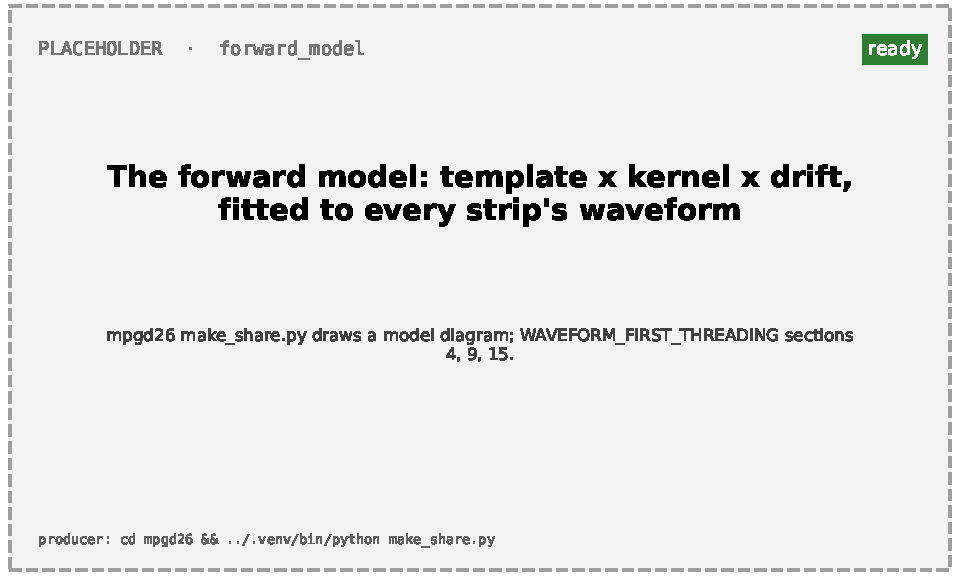
\includegraphics[width=0.9\linewidth]{forward_model}
  \caption{\tbw{The forward model.}}
  \label{fig:forward_model}
\end{figure}

\section{The physics floor}\label{sec:floor}
\sectionstate{partial}{toy closure, WFT \S12 (\texttt{18\_toy\_closure.py}, R\&D model)}
\intent{What limits the angle once the bias is gone: electronics contribute 0.02\textdegree; $\sim$1\textdegree{} comes from
the 0.3\,mm jitter of the charge centroid (diffusion). The floor is physics, not readout.}
\analysis{R6}{re-run the toy on the production model and the r06 kernel}
\begin{figure}[t]
  \centering
  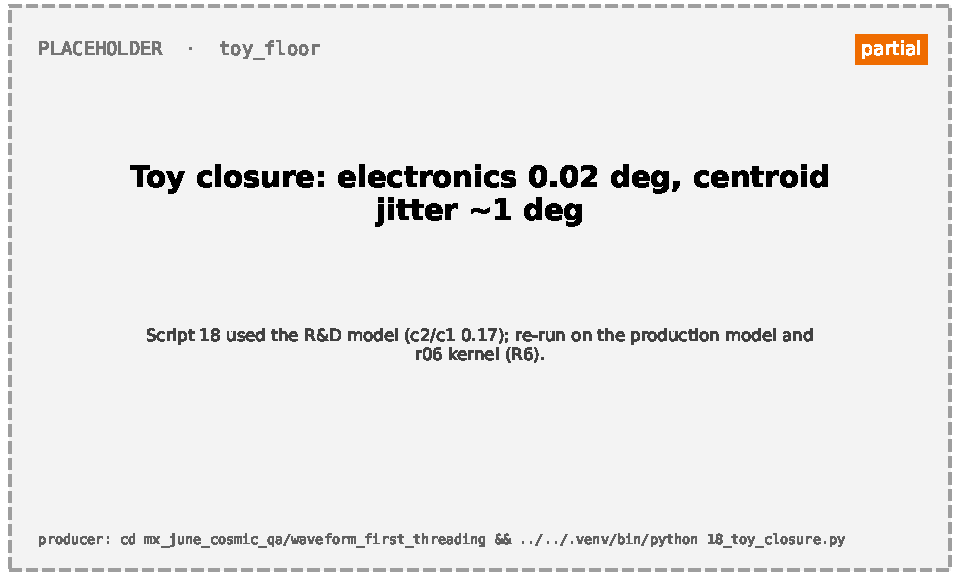
\includegraphics[width=0.7\linewidth]{toy_floor}
  \caption{\tbw{Toy closure: contributions to the angular resolution.}}
  \label{fig:toy_floor}
\end{figure}

\section{Hits against waveforms, same events}\label{sec:tiers}
\sectionstate{open}{R1--R5; the July det3 five-tier table (R\&D model); FLEET\_DIGEST (H0 vs W)}
\intent{The core new result. Every tier on the same events with the same reference: H0 production hits, H1 best
per-strip estimator, H2a slope remap, H2b unsharing + angle-calibrated hybrid, H2c the forward model fitted to hit
lists, W waveforms. Metrics: $\sigma_\theta$ vs angle, bias, implied-$v$ flatness, threading $<1$\,mm, position, efficiency, near-vertical tracks.}
\analysis{R2}{H2a/H2b refitted on r06}
\analysis{R3}{H2c: forward fit on hit lists}
\analysis{R5}{benchmark, all tiers}
\begin{figure}[t]
  \centering
  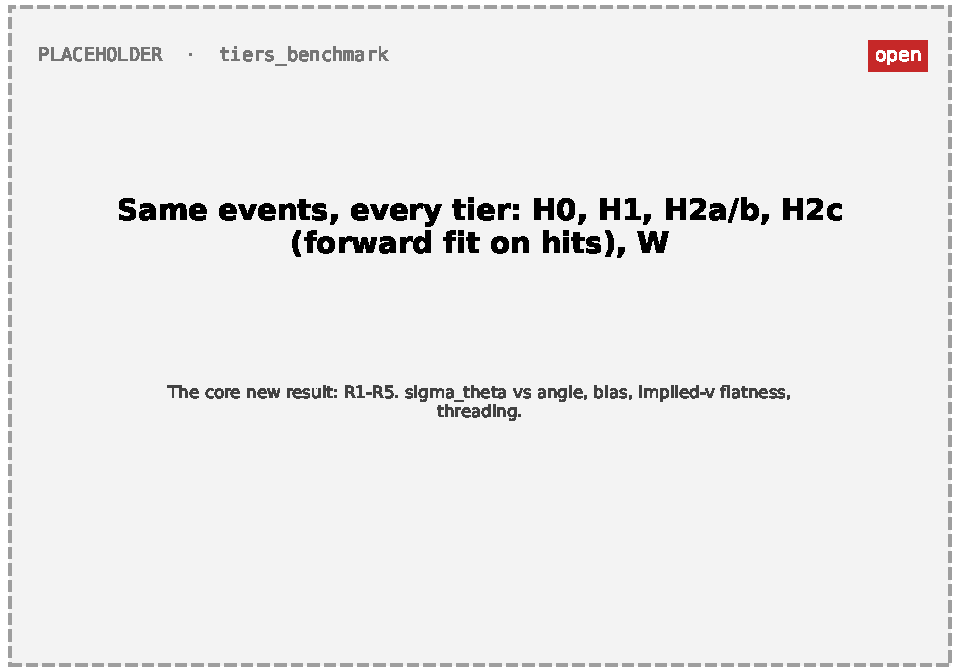
\includegraphics[width=0.95\linewidth]{tiers_benchmark}
  \caption{\tbw{Every reconstruction tier on the same events.}}
  \label{fig:tiers_benchmark}
\end{figure}

\section{What a hit readout must record}\label{sec:readout}
\sectionstate{open}{R4; VMM emulation deferred (V1, \texttt{ntof\_cosmics/g4\_digi})}
\intent{For a hit-only front-end: which threshold, whether to read $\pm1/\pm2$ neighbours, whether to keep amplitude.
Answered in general terms; a full VMM emulation is left for later.}
\analysis{R4}{threshold 3--7$\sigma$, neighbour readout, amplitude on/off}
\begin{figure}[t]
  \centering
  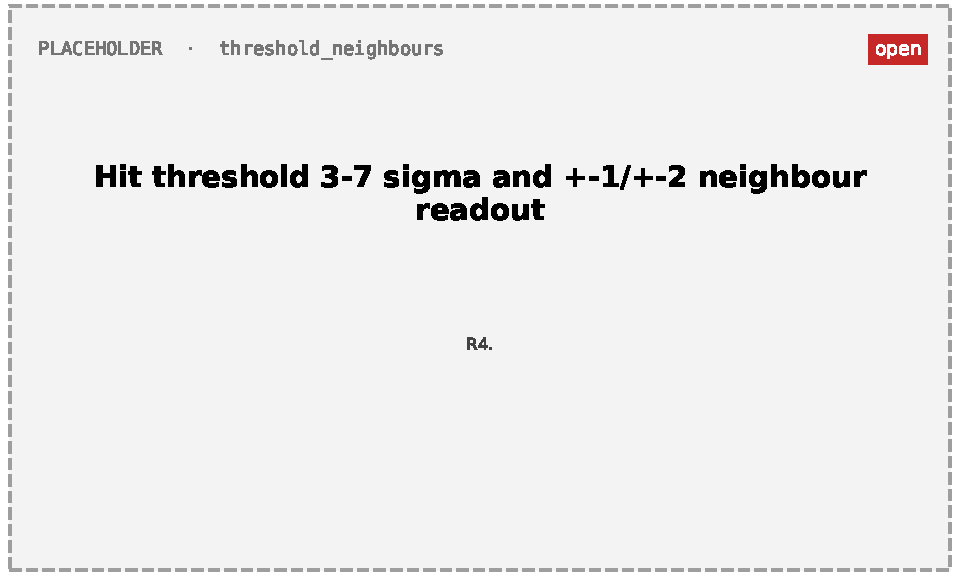
\includegraphics[width=0.75\linewidth]{threshold_neighbours}
  \caption{\tbw{Angular resolution against hit threshold and neighbour readout.}}
  \label{fig:threshold_neighbours}
\end{figure}

\section{A known angle in the beam}\label{sec:knownangle}
\sectionstate{open}{R7; \texttt{sps\_beam\_test\_26/analysis/angled\_kernel} (geometry)}
\intent{A reference-free test: det4 rotated by 25.6\textdegree{} in the SPS beam. Hits and waveforms against the stage angle,
independent of the M3 telescope.}
\analysis{R7}{known-angle reconstruction, hits vs waveforms}
\begin{figure}[t]
  \centering
  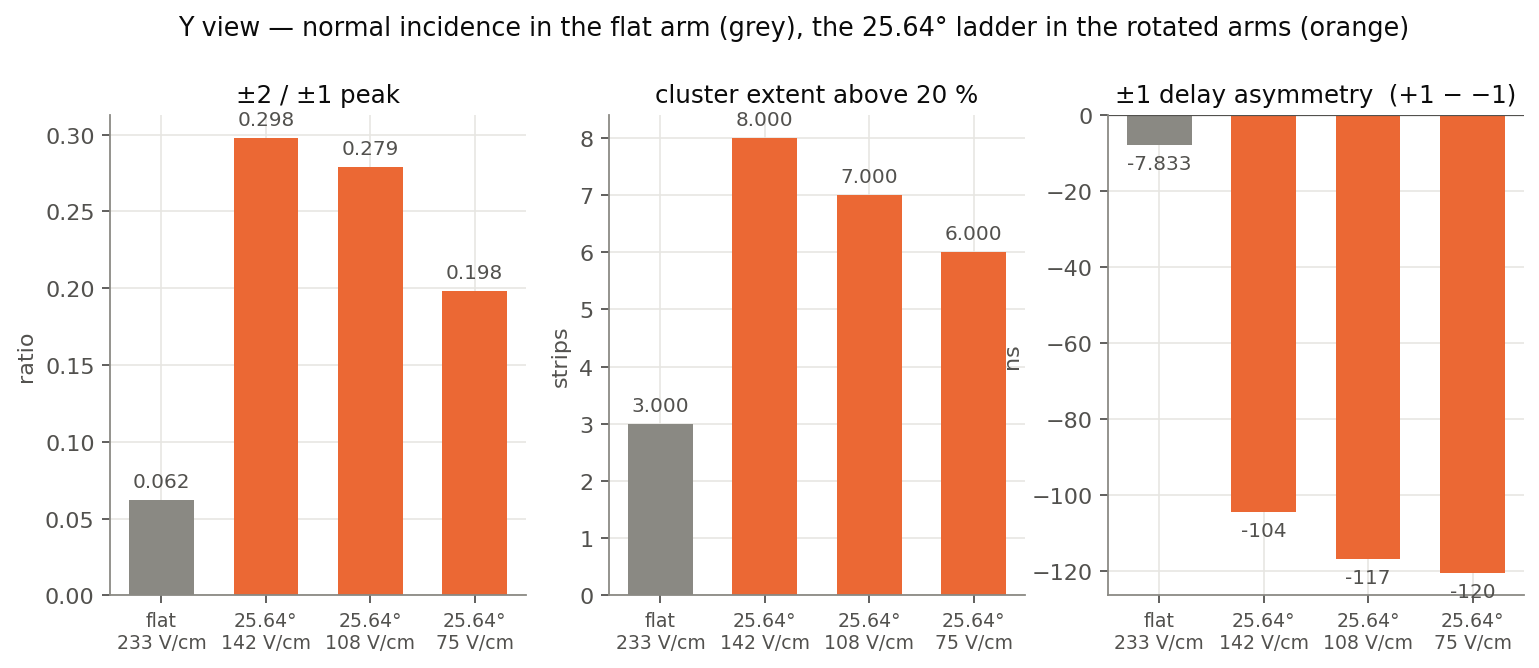
\includegraphics[width=0.6\linewidth]{known_angle_geometry}
  \caption{\tbw{det4 rotated in the beam.}}
  \label{fig:known_angle_geometry}
\end{figure}
\begin{figure}[t]
  \centering
  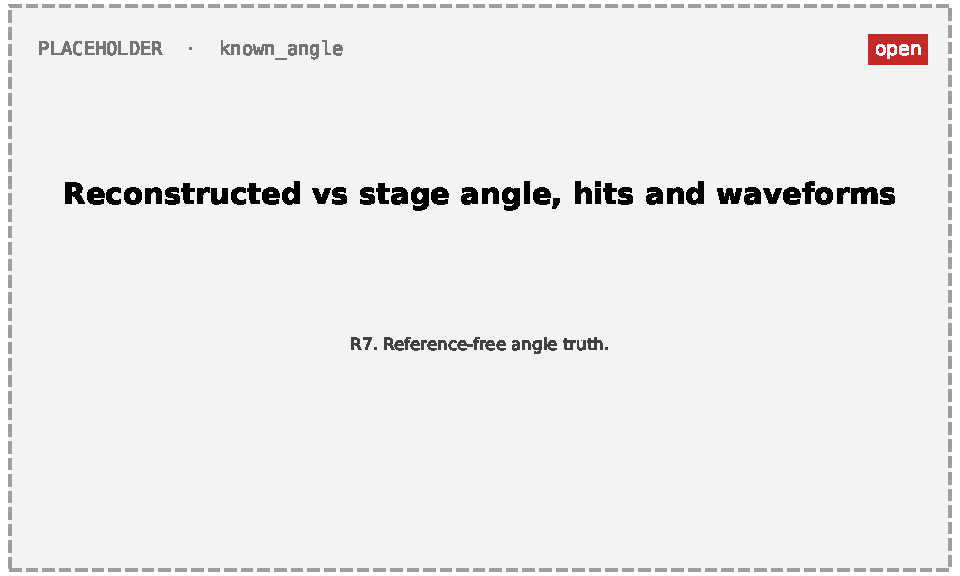
\includegraphics[width=0.7\linewidth]{known_angle}
  \caption{\tbw{Reconstructed angle against the stage angle.}}
  \label{fig:known_angle}
\end{figure}

\section{Fleet performance, cost and outlook}\label{sec:fleet}
\sectionstate{partial}{\texttt{mx\_june\_wft/FLEET\_DIGEST.md}; R10 (cost table)}
\intent{All five chambers: $\sigma_\theta$ = \requote{1.15--2.51\textdegree} with waveforms, better than hits on every plane
(\requote{$\times$1.03--2.2}, halved on det3). CPU cost per plane and tier. Outlook: VMM emulation, in-situ calibration at n\_TOF, two-track fits.}
\analysis{R10}{cost table}
\analysis{C3}{n\_TOF tripwires: chamber C non-linearity on its own bundle}
\begin{figure}[t]
  \centering
  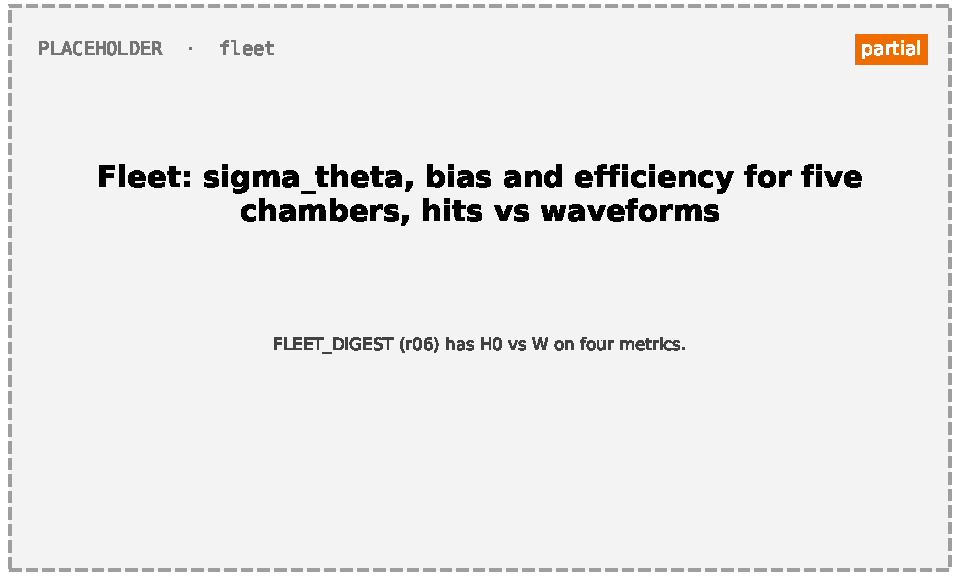
\includegraphics[width=0.9\linewidth]{fleet}
  \caption{\tbw{Fleet performance, hits against waveforms.}}
  \label{fig:fleet}
\end{figure}

\section{Conclusions}\label{sec:conclusions}
\sectionstate{open}{all of the above}
\tbw{The bias, its cause, the fix, what it costs, and what a hit readout would need.}


\bibliographystyle{unsrt}
\bibliography{refs}
\end{document}
